\chapter{Main window controls}
\minitoc  


See Fig. \ref{gui} to have an overview of the controls described in this chapter.

%\section{Open and save data }
%\section{Undo and redo actions }


 \section{Camera controls}
Most camera related controls lay on the left part of the main window. See Fig. \ref{gui} to find the location of the "Camera" controls in the main Window.
\subsection{Camera rotation center}
By default, the camera rotates around the origin of the coordinate system (x=0, y=0, z=0), but by pressing ``
\includegraphics[scale=0.7]{images/06/camera/move_cam.png}"/``\includegraphics[scale=0.7]{images/06/camera/move_cam2.png}", the camera will revolve around the center of mass of all opened objects. The latter option is useful when the centre of mass of an object (or of several ones) is far from the origin of the coordinate system. The grid is drawn using different colors depending on the camera rotation centre (see Fig. \ref{grid_color}). %The camera centre can also be set at the location of one of the first 10 ``normal" landmarks (see section \ref{camera_centre_at}).

\begin{figure}
  \centering
  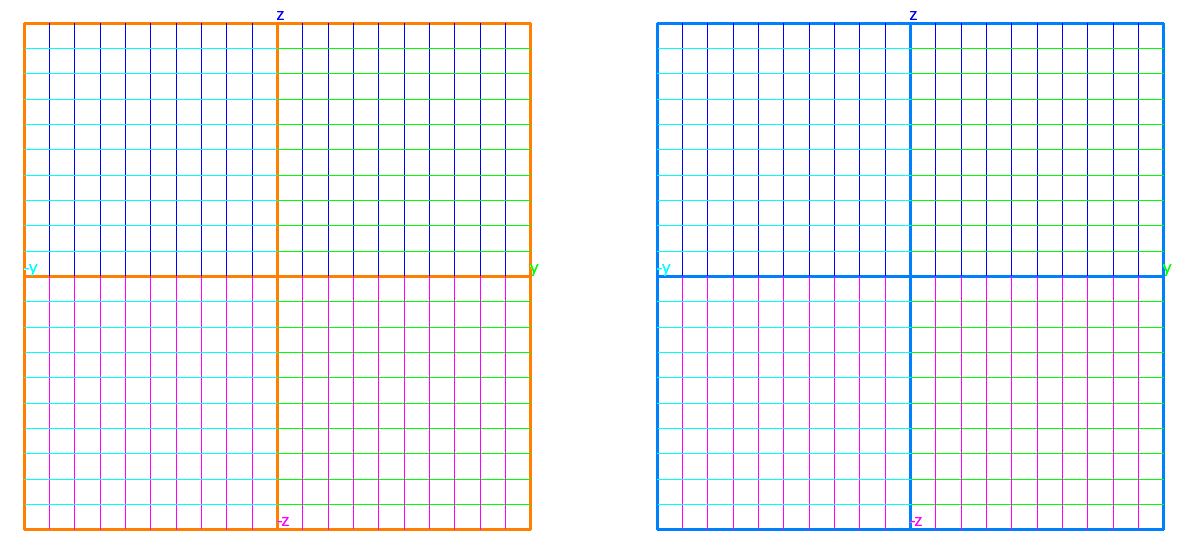
\includegraphics[scale=0.4]{images/06/camera/grids.png} 
	\caption{Grid display color. Left: when the camera revolves around the origin of the coordinate system (x=0, y=0, z=0), the grid outline is displayed in orange. Right: when the camera revolves around the center of mass of all opened objects, the grid has a blue outline.}
\label{grid_color}
 
\end{figure}

 
\subsection{Orthographic or perspective camera projection}
You can switch between orthographic and perspective projection mode by pressing the "
\includegraphics[scale=0.7]{images/06/camera/camera_ortho.png}" or "
\includegraphics[scale=0.7]{images/06/camera/camera_persp}" toggle button (see also see Fig. \ref{camera_ortho_example}).
Note that in orthographic camera projection mode 
\includegraphics[scale=0.7]{images/06/camera/camera_ortho.png}, when the grid is displayed, the relationship between pixel size on the screen and real world dimensions appears on the right bottom corner of the screen: 
\includegraphics[scale=0.7]{images/06/camera/grid_infos.png}. 

\begin{figure}
  \centering
  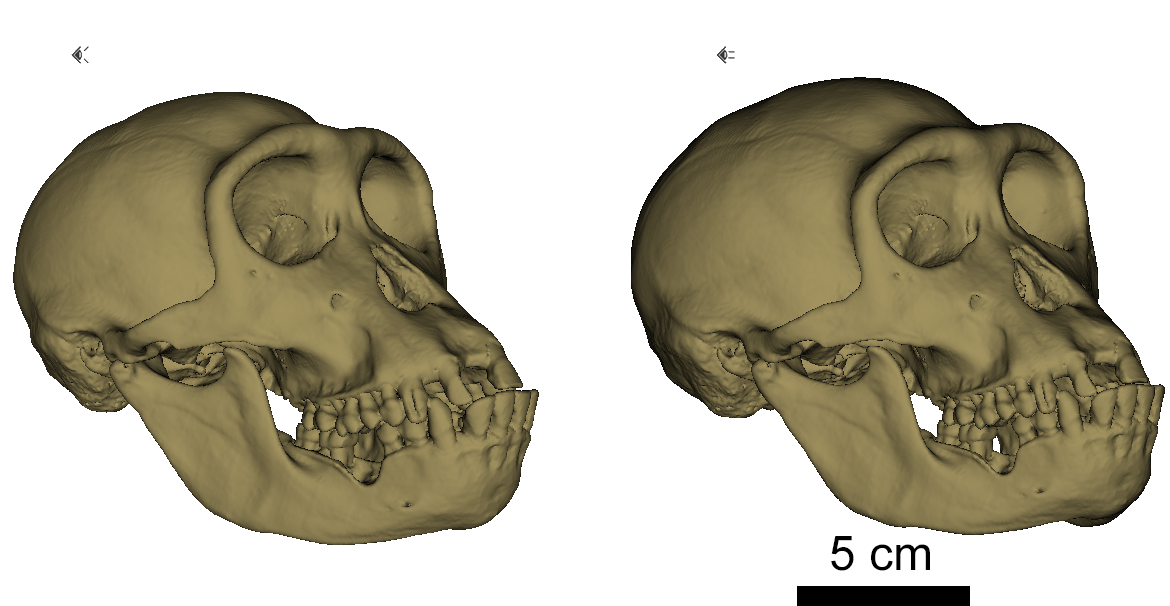
\includegraphics[scale=0.4]{images/06/camera/camera_ortho_example.png} 
	\caption{Perspective and Orthographic camera projection modes. Skull of \textit{Pan paniscus}. Left: perspective camera projection mode: closer structures appear larger than farther structures. Right: orthographic camera projection mode: a uniform relation exists between pixel size and real world dimensions, making it possible to place a scale bar. }
\label{camera_ortho_example}
 
\end{figure}


\subsection{Camera orientation}
6 camera positions are predefined :\\

\includegraphics[scale=0.7]{images/06/camera/camera_right.png} view object from right side \\

\includegraphics[scale=0.7]{images/06/camera/camera_left.png} view object from left side\\

\includegraphics[scale=0.7]{images/06/camera/camera_front.png} view object from front side (default camera position)\\

\includegraphics[scale=0.7]{images/06/camera/camera_back.png} view object from back side\\

\includegraphics[scale=0.7]{images/06/camera/camera_above.png} view object from above\\

\includegraphics[scale=0.7]{images/06/camera/camera_below.png} view object from below\\

\subsection{Camera rotation around ``z" viewing axis}

\begin{minipage}{0.7\textwidth}
To do so, you may use the slider lying around the center of the left panel of the main window.
\end{minipage}    
\begin{minipage}{0.25\textwidth}\centering
  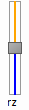
\includegraphics[scale=0.7]{images/06/camera/rz_cam.png}
 \captionof{figure}{Camera ``z" rotation slider}
 \end{minipage}    



\subsection{Clipping plane slider}

\begin{minipage}{0.7\textwidth}
In some cases, you may need to displace the viewing clipping plane. To do so, use
the slider lying centrally in the left panel of the main window. See \ref{Clipping_plane} for additional clipping plane functionalities.\\

\end{minipage}    
\begin{minipage}{0.25\textwidth}\centering
  
\includegraphics[scale=0.5]{images/06/camera/cp_slider.png}
 \captionof{figure}{Camera clipping plane slider}
 \end{minipage}   




\subsection{Zoom}
There are three main ways to modify the ``zoom" in MorphoDig :


\begin{minipage}{0.7\textwidth}
\begin{itemize}
\item You may use the zoom slider laying in the lower part of the left panel of the main window.
\item	You may set manually the display scale (Edit $\rightarrow$  Edit size unit and grid spacing, then define the display scale: 100 pixels in size unit). This option is only available in orthographic projection mode 
\includegraphics[scale=0.7]{images/06/camera/camera_ortho.png}.
\item	You may use the middle click mouse roll button (roll the wheel).
\end{itemize}
\end{minipage}    
\begin{minipage}{0.25\textwidth}\centering
  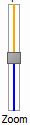
\includegraphics[scale=0.7]{images/06/camera/zoom_slider.png}
 \captionof{figure}{Zoom slider}


 \end{minipage}    


\section{Display controls}
The display controls mentioned in this section are situated on the top part of the main window (see Fig. \ref{gui}).


\subsection{Grid}
Press 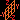
\includegraphics[scale=0.7]{images/06/display/grid.png} to show / hide the grid. Default grid size is 1 cm / square. Grid size can be edited manually
(viewing opt. $\rightarrow$ Grid size).
Switching between the 6 camera predefined positions defined above (
\includegraphics[scale=0.7]{images/06/camera/camera_right.png}, 

\includegraphics[scale=0.7]{images/06/camera/camera_left.png}, 

\includegraphics[scale=0.7]{images/06/camera/camera_front.png}, 

\includegraphics[scale=0.7]{images/06/camera/camera_back.png}, 

\includegraphics[scale=0.7]{images/06/camera/camera_above.png} and 

\includegraphics[scale=0.7]{images/06/camera/camera_below.png})
will affect the plane in which the grid is drawn.




\subsection{Coordinate system orientation helper}
\begin{minipage}{0.7\textwidth}
Press 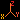
\includegraphics[scale=0.7]{images/06/display/orientation_helper.png} to show / hide the coordinate system orientation helper lying on the bottom left corner of the main 3D window. By default, the labels are defined
the following way:\\
+z axis : dorsal side\\
-z axis : ventral side\\
+y axis : left side\\
-y axis : right side\\
+x axis : anterior side\\
-x axis : posterior side.\\
You may edit these labels depending on your preferences (for instance,
depending on the structure you are working with, you may need to set ``+y" to ``labial", and ``-y" to
``lateral"). To edit orientation labels, click on ``Edit $\rightarrow$ Edit orientation labels."
\end{minipage}    
\begin{minipage}{0.3\textwidth}\centering
 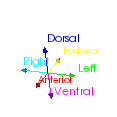
\includegraphics[scale=0.7]{images/06/camera/orientation_helper_view.png}
 \captionof{figure}{Orientation helper}
 \end{minipage}   


\subsection{Anaglyph}
Press 
\includegraphics[scale=0.7]{images/06/display/anaglyph.png} to activate/deactivate anaglyph 3D rendering.
See Fig. \ref{anaglyph_example}. You then need to wear "Red/Blue" 
\includegraphics[scale=0.7]{images/06/display/anaglyph_glasses.png} glasses to visualize objects in 3D.

\begin{figure}
  \centering
  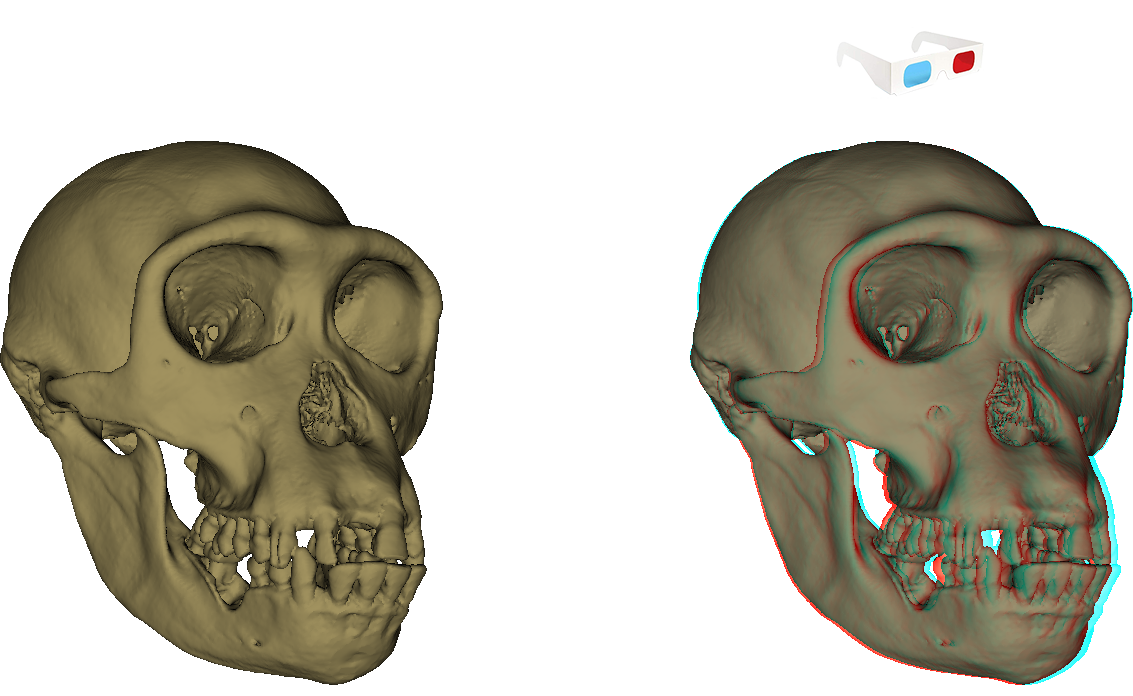
\includegraphics[scale=0.34]{images/06/display/anaglyph_example.png} 
	\caption{Anaglyph display mode. Left: normal display mode. Right: anaglyph display mode. Cranium of the holotype specimen of \textit{Pan paniscus}.}
\label{anaglyph_example}
 
\end{figure}



%You can also modify the clipping plane manually by editing the ``Tz" control in the camera options window (viewing opt. $\rightarrow$ Camera $\rightarrow$ Camera options).

\subsection{Clipping plane} \label{Clipping_plane}

The button 
\includegraphics[scale=0.7]{images/06/display/cpon.png} or 
\includegraphics[scale=0.5]{images/06/display/cpoff.png}  permits to adjust / readjust the position of the clipping plane at predefined positions (see for instance Fig. \ref{cp_example}):
\begin{itemize}
\item  
\includegraphics[scale=0.7]{images/06/display/cpon.png}: the clipping plane is placed at z = 0 (all objects having a z coordinate along
z viewing axis smaller than 0 are hidden).
\item	
\includegraphics[scale=0.7]{images/06/display/cpoff.png} : the clipping plane is replaced at its original value : z= - camera.far / 2. This value permits to
view objects having positive and negative coordinates along z viewing axis.

\end{itemize}
\begin{figure}
  \centering
  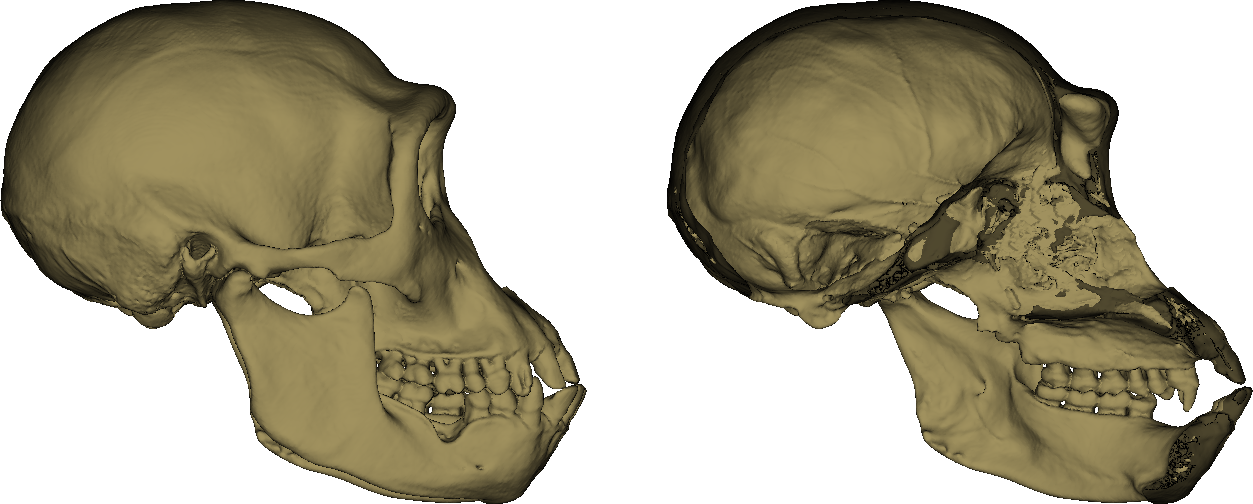
\includegraphics[scale=0.4]{images/06/display/cp_example.png} 
	\caption{Clipping plane display mode. Cranium of the type specimen of \textit{Pan paniscus}. Left: normal display mode. Right: clipping plane display mode "on" : permits to visualize inner structures. }
\label{cp_example}
 
\end{figure}



\subsection{Backface culling} \label{Backface_culling}

Hiding backfaces of a surface is useful in some cases to visualize inner structures of a biological object (see for instance Fig. \ref{backface_example}). The button 
\includegraphics[scale=0.7]{images/06/display/backface_on.png} / 
\includegraphics[scale=0.7]{images/06/display/backface_off.png}  permits to visualize/hide backfaces :
\begin{itemize}
\item  
\includegraphics[scale=0.7]{images/06/display/backface_on.png}: both sides of a given surface object are rendered.
\item	
\includegraphics[scale=0.7]{images/06/display/backface_off.png} : backfaces are hidden (only frontfaces are visible).

\end{itemize}


\begin{figure}
  \centering
  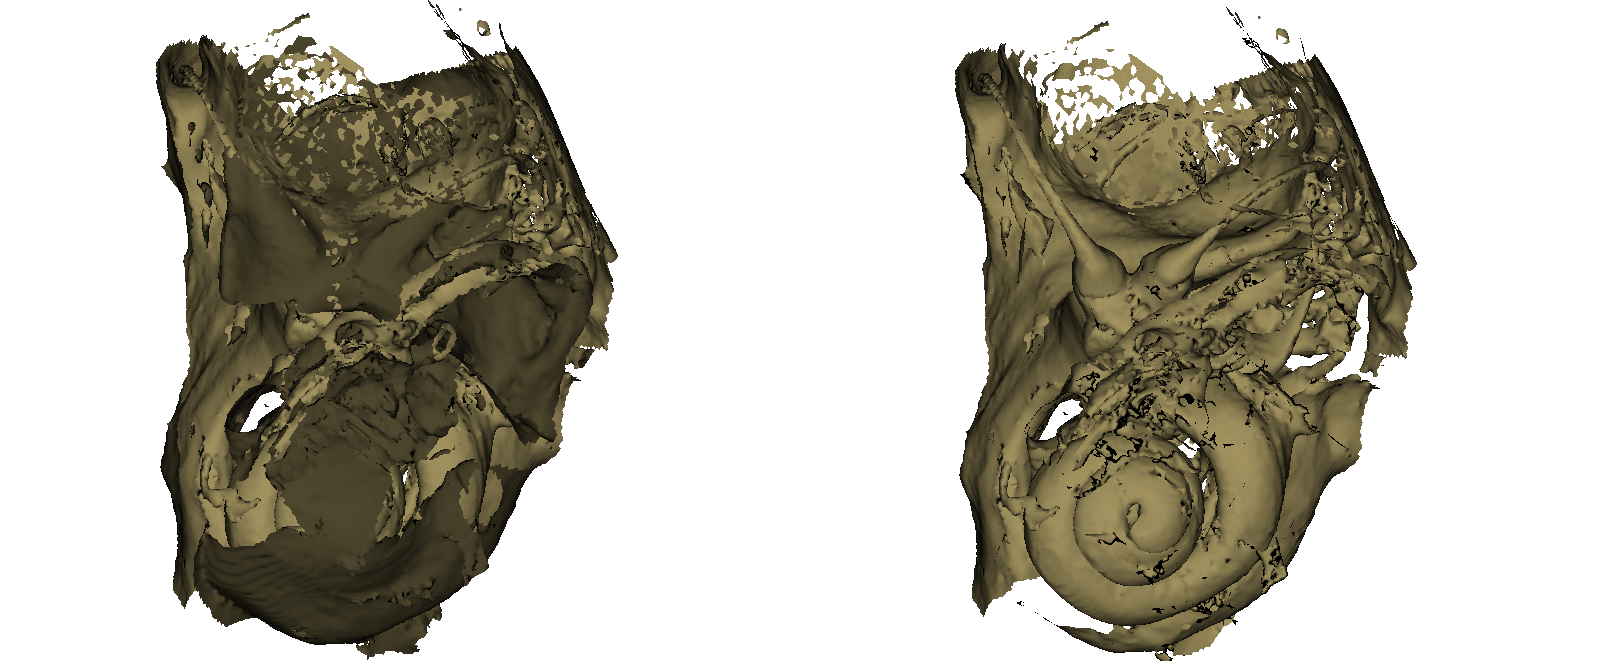
\includegraphics[scale=0.3]{images/06/display/backface_example.png} 
	\caption{Backface culling display mode. Petrosal bone of \textit{Eulemur mongoz}. Left: normal display mode: both frontfaces (lighter) and backfaces (darker) are displayed. Right: backface culling mode activated: only frontfaces are displayed, making it easier to visualize the bony labyrinth. }
\label{backface_example}
 
\end{figure}



\subsection{Surface 3D representation controls}


4 different options exist to draw 3D surfaces :\\

\includegraphics[scale=0.7]{images/06/display/point_normals.png} : point normales display mode (Gouraud shading)\\

\includegraphics[scale=0.7]{images/06/display/cell_normals.png} : triangle normales display mode \\

\includegraphics[scale=0.7]{images/06/display/wireframe.png} : wireframe representation  display mode\\

\includegraphics[scale=0.7]{images/06/display/points.png} point cloud display mode \\


\section{Light direction controls}
See Fig. \ref{gui} to see where the "light controls" are situated within MorphoDig's main window.


6 lightning orientations are predefined :\\

\includegraphics[scale=0.7]{images/06/light/light_right.png}light from right viewing side\\

\includegraphics[scale=0.7]{images/06/light/light_left.png}light from left viewing side\\

\includegraphics[scale=0.7]{images/06/light/light_front.png}light from front viewing side\\

\includegraphics[scale=0.7]{images/06/light/light_back.png}light from back viewing side\\

\includegraphics[scale=0.7]{images/06/light/light_above.png}light from above\\

\includegraphics[scale=0.7]{images/06/light/light_below.png}light from below\\




  \section{Object controls}
See Fig. \ref{gui} to see where the "object controls" are situated within MorphoDig's main window. Remind that only selected objects are affected by these controls.

\subsection{Delete selected objects}
Clicking on "\includegraphics[scale=0.7]{images/06/objects/delete2.png}" deletes all selected objects. This action can be undone/redone.

\subsection{Create landmark at X,Y,Z}
Clicking on "\includegraphics[scale=0.7]{images/06/objects/landmark_xyz.png}" opens the "Create landmark" window  (Fig. \ref{create_landmark}), in which a new landmark can be created a specified coordinates. This action can be undone/redone..

\begin{figure}
  \centering
  \includegraphics[scale=0.55]{images/06/objects/create_landmark.png} 
	\caption{Create landmark at a given X,Y,Z coordinate.}
\label{create_landmark}
 
\end{figure}
\subsection{Decrease / Increase landmark number}
Clicking on \includegraphics[scale=0.7]{images/06/objects/move_up.png} will increase (if possible) the landmark number of all selected landmarks. Clicking on \includegraphics[scale=0.7]{images/06/objects/move_down.png} will decrease (if possible) the landmark number of all selected landmarks. These button make it possible to reorder landmarks.
\subsection{Edit first selected surface}

Clicking on "\includegraphics[scale=0.7]{images/06/objects/actor_edit.png}" opens the "Edit first selected surface" window (Fig. \ref{actor_edit}), in which several properties of a given surface object can be edited.
\\
- Object name : modifies the name of the object.\\
- Next object \includegraphics[scale=0.7]{images/06/objects/s_right.png} and preceding object \includegraphics[scale=0.7]{images/06/objects/s_left.png}: saves currently  settings and fetches next/preceding surface.\\
- Object solid color : modifies the "solid color" property of this object.\\
- Object translucency : modifies the translucency this object.
- Object matrix : current position/rotation matrix of the object.\\
- Reinit matrix: set current matrix to identity.\\
- Apply matrix to all selected surfaces : set position/rotation matrix to all other selected surfaces.\\
- Existing arrays : list of all scalar/RGB color/tags arrays associated to the vertices of the surfaces.\\
- Edit array name : modifies the name of currently selected array\\
- Duplicate array : duplicates currently selected array\\
- Delete array : deletes currently selected array\\
- Ok : save settings and closes window



\begin{figure}
  \centering
  \includegraphics[scale=0.55]{images/06/objects/edit_surface.png} 
	\caption{Edit first selected surface window.}
\label{actor_edit}
 
\end{figure}



\subsection{Edit first selected landmark}
Clicking on "\includegraphics[scale=0.7]{images/06/objects/landmark_edit.png}" opens the "Edit first selected landmark" window (Fig. \ref{landmark_edit}), in which landmark coordinates of landmarks can be manually edited. The center of rotation of the camera can be set to the x,y,z coordinates of a given landmark by pressing on "\includegraphics[scale=0.7]{images/06/objects/move_cam3.png}".




\begin{figure}
  \centering
  \includegraphics[scale=0.55]{images/06/objects/edit_landmark.png} 
	\caption{Edit first selected landmark window.}
\label{landmark_edit}
 
\end{figure}

\subsection{Edit first selected flag}
Clicking on "\includegraphics[scale=0.7]{images/06/objects/flag_edit.png}" opens the "Edit first selected landmark" window (Fig. \ref{flag_edit}), in which several properties of a given flag can be manually edited.

- Flag name : modifies the label of this flag.\\
- X, Y, Z: 3D coordinates of the flag.\\
- Next flag \includegraphics[scale=0.7]{images/06/objects/s_right.png} and preceding flag \includegraphics[scale=0.7]{images/06/objects/s_left.png}: saves currently  settings and fetches next/preceding flag\\
- Flag color : modifies the "color" of the currently selected flag.\\
- Flag rendering size : modifies the length of the flag.\\
The center of rotation of the camera can be set to the x,y,z coordinates of a given flag by pressing on "\includegraphics[scale=0.7]{images/06/objects/move_cam3.png}".


\begin{figure}
  \centering
  \includegraphics[scale=0.55]{images/06/objects/edit_flag.png} 
	\caption{Edit first selected flag window.}
\label{landmark_edit}
 
\end{figure}
\subsection{Lasso cut selected surfaces} \label{lasso_cut_section}

You may cut through an input selected surface using this option (see Fig. \ref{lasso_cut}). Once "\includegraphics[scale=0.7]{images/06/objects/lasso_keepinside.png}" (lasso cut keep inside) or "\includegraphics[scale=0.7]{images/06/objects/lasso_keepoutside.png}" (lasso cut keep outside) has been pressed, the mouse cursor changes and you can start drawing the lasso section by dragging the mouse while the left button is pressed. When the left button is released, the lasso cut operation starts: a new object is created, which contains all the parts of the selected object laying inside or outside the drawn polygon, respectively.\\

\begin{figure}
  \centering
  \includegraphics[scale=0.6]{images/06/objects/lasso_cut.png} 
	\caption{A: "Lasso keep outside" button is pressed, then a polygon is drawn over the selected object (grey) by maintaining left mouse button pressed and dragging the mouse. B: Left mouse button has been released : a new surface object is  created. C: "Delete" has been pressed : only the newly created  object remains. C: "Lasso keep inside" is pressed, then a polygon is drawn over the selected object (grey) by maintaining left mouse button pressed and dragging the mouse. E: Left mouse button has been released : a new surface object is  created. F: "Delete" has been pressed : only the newly created  object remains. }
\label{lasso_cut}
 
\end{figure}




\subsection{object rotation and translation sliders}
	As seen earlier, selected objects can be translated and rotated using the mouse left and middle buttons
(in landmark and camera selection modes, you also need to maintain ``CTRL" button pressed
while dragging the mouse to achieve rotation and translation of selected objects). Alternatively, you
may also use the following controls to accomplish rotation and translation of selected objects. Rotation
is performed around the global center of mass of all currently selected objects.

\subsubsection{Rotation around and translation along ``Z" viewing axis }

These controls are extremely useful, as there is no way to achieve rotation round « z » viewing axis or translation along ``z" viewing axis using the
mouse. \\ To do so, use the tz and rz sliders (see Fig. \ref{move_z}).


\begin{figure}
  \centering
  \includegraphics[scale=0.45]{images/06/objects/move_objects_z.png} 
	\caption{A: object and tz slider are in initial position. B: tz slider is moved down: the selected object moves forward. C: tz slider is moved up. The selected object moves backward. D: object and rz slider are in initial position. E: rz slider is moved down: the selected object rotates around the "roll" axis counter-clockwise. F: rz slider is moved up. The selected object rotates around the "roll" axis clockwise.}
\label{move_z}
 
\end{figure}



\subsubsection{Rotation/translation around/along ``Y" viewing axis}

To do so, use the ty and ry sliders (see Fig. \ref{move_y}).

\begin{figure}
  \centering
  \includegraphics[scale=0.45]{images/06/objects/move_objects_y.png} 
	\caption{A: object and ty slider are in initial position. B: ty slider is moved down: the selected object moves downward. C: ty slider is moved up. The selected object moves upward. D: object and ry slider are in initial position. E: ry slider is moved down: the selected object rotates around the "yaw" axis clockwise. F: ry slider is moved up. The selected object rotates around the "yaw" axis counter-clockwise.}
\label{move_y}
 
\end{figure}



\subsubsection{Rotation/translation around/along ``X" viewing axis}

To do so, use the ty and ry sliders (see Fig. \ref{move_x}).

\begin{figure}
  \centering
  \includegraphics[scale=0.45]{images/06/objects/move_objects_x.png} 
	\caption{A: object and tx slider are in initial position. B: tx slider is moved down: the selected object moves leftward. C: tx slider is moved up. The selected object moves rightward. D: object and rx slider are in initial position. E: rx slider is moved down: the selected object rotates around the "pitch" axis clockwise. F: rx slider is moved up. The selected object rotates around the "pitch" axis counter-clockwise.}
\label{move_x}
 
\end{figure}